\renewcommand{\baselinestretch}{2} \small\normalsize
\chapter{RADAR Basics}
This chapter covers some RADAR basics, including the RADAR ranage equation, bistatic configurations, antenna beam widths and a summary of threshold detection.

\section{RADAR Range Equation} 
The RADAR range equation provides a deterministic method to calculate received signal levels and is the workhorse for analyzing RADAR system performance. This equation is the first step towards building a statistical model, as it captures the underlying physics.

\subsection{Monostatic Case}
The RADAR range equation is derived by assuming spherically propagating waves and computing the propagated power at 4 incremental points between the transmitter and target as shown in Figure \ref{intro_fig:1}. These points are the projected power ($P_1$), the power received at the target ($P_2$), the power reflected by the target ($P_3$), and the power at the receiver antenna ($P_4$). The received power ($P_r$) is then the product of $P_4$ and the effective area of the receiver antenna.

\begin{figure}[H]
  \begin{center}
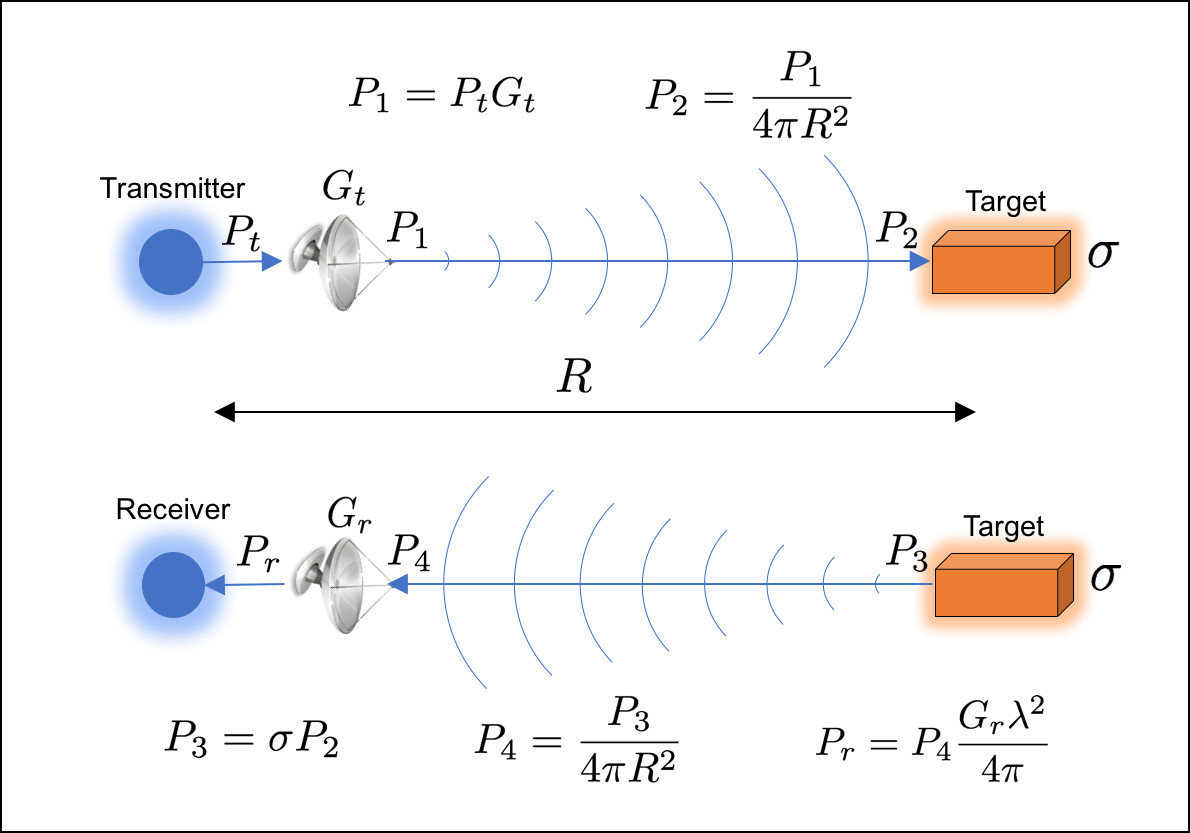
\includegraphics[width=4in]{../media/multistatic/radar_range_equation.png}
  \end{center}
  \renewcommand{\baselinestretch}{1} \small\normalsize
  \begin{quote}
    \caption[RADAR Range Equation Derivation]{RADAR Range Equation Derivation \label{intro_fig:1}}
  \end{quote}
\end{figure}
\renewcommand{\baselinestretch}{2} \small\normalsize

With spherical waves, the power is spread out over a sphere of radius equal to the slant range, $R$, which gives the scaling factor of $\left( 4\pi R^2 \right)^{-1}$. The total projected power is the transmitted power, $P_t$, multiplied by the antenna gain, $G_t$. The RADAR cross section (RCS), $\sigma$, defines the amount of power reflected. The effective area of the antenna is then $\frac{G_t\lambda^2}{4\pi}$.

In the monostatic case, $G_t = G_r$ and the RADAR range equation is given in Equation \ref{intro_eq:1}.
  \begin{equation}
  \label{intro_eq:1}
 P_r = \frac{P_tG_t^2\sigma\lambda^2}{\left(4\pi\right)^3R^4}
  \end{equation}
In this equation, the antenna gain, $G_t$ is a function of the angle between the antenna boresight and the target. Randomness enters this version of the RADAR range equation through this angle and the target RCS, $\sigma$.

In the atmosphere, propagation is a linear operation. Therefore we can leverage superposition to compute the RADAR range equation for each path or scatterer and sum the results.

We can divide Equation \ref{intro_eq:1} by the noise power to represent the RADAR equation in terms of signal to noise ratio (SNR) as shown in Equation \ref{intro_eq:2} \cite{skolnik_handbook}.
\begin{equation}
    \label{intro_eq:2}
\text{SNR} = \frac{P_r}{P_n} = \frac{P_tG_t^2\sigma\lambda^2}{\left(4\pi\right)^3 R^4k_BTBF_n}
\end{equation}
In this equation, $k_B$ is the Boltzmann constant, $B$ is the receiver bandwidth, $T$ is the receiver temperature and $F_n$ is the receiver noise figure. Nominally, $B$ is taken to be the inverse of the pulse width to accomodate matched filter processing and $T$ is taken to be $300$ K.

\subsection{Bistatic Case}
In the bistatic case, we need to consider each path separately as the ranges, antenna gains, and RCS are all likely different. The standard bistatic RADAR range equation is shown in Equation \ref{intro_eq:3}.
  \begin{equation}
  \label{intro_eq:3}
 P_r = \frac{P_tG_tG_r\sigma_B\lambda^2}{\left(4\pi\right)^3R_1^2R_2^2}
  \end{equation}
In this equation, $G_t$ is the antenna gain for the transmitter, $G_r$ is the antenna gain for the receiver, $\sigma_B$ is the bistatic RCS, $R_1$ is the slant range along the first path (transmitter to target), and $R_2$ is the slant range along the second path (target to receiver). Again, the antenna gains, $G_t$ and $G_r$ are functions of the angle between the antenna boresight and the target.

The bistatic RADAR range equation in terms of SNR is shown in Equation \ref{intro_eq:4}.
\begin{equation}
    \label{intro_eq:4}
\text{SNR} = \frac{P_tG_tG_r\sigma_B\lambda^2}{\left(4\pi\right)^3 R_1^2R_2^2k_BTBF_n}
\end{equation}

\subsection{Propagation Factors}
The use of a propagation factor, $F_p$, allows us to include atmospheric effects in the RADAR range equation. These effects can include absorption from atmospheric gases and weather such as rain or snow as well as rollups for the effects of multipath reflections, diffraction from the surface, and clipping by the horizon. The propagation factor is typically implemented as a multiplier to the RADAR range equation and is generally complicated to compute. 

The bistatic RADAR range equation with a propagation factor included in given in Equation \ref{intro_eq:4a}.
  \begin{equation}
  \label{intro_eq:4a}
 P_r = \frac{P_tG_tG_r\sigma_B\lambda^2}{\left(4\pi\right)^3R_1^2R_2^2}F_p
  \end{equation}
The propagation factor provides another mechanism to introduce randomness.

\section{Bistatic Configurations}

\begin{figure}[H]
  \begin{center}
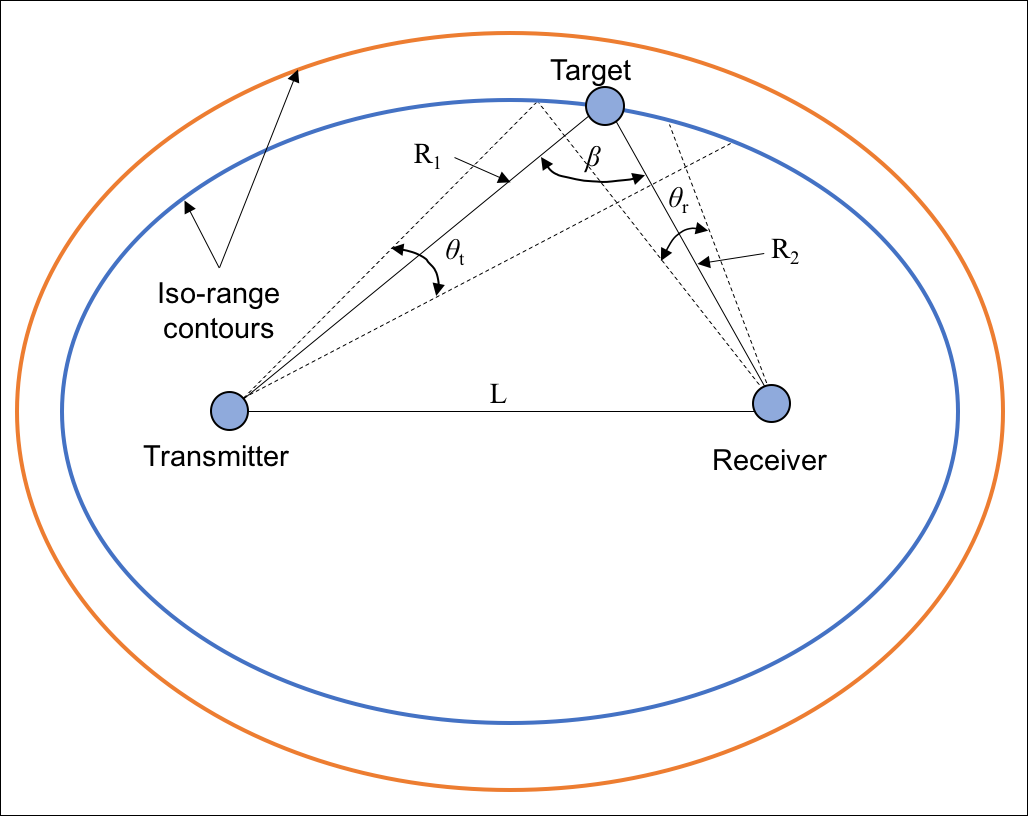
\includegraphics[width=4in]{../media/multistatic/Isorange_contours.png}
  \end{center}
  \renewcommand{\baselinestretch}{1} \small\normalsize
  \begin{quote}
    \caption[Isorange Contours for Bistatic Configuration]{Isorange Contours for Bistatic Configuration \label{intro_fig:2}}
  \end{quote}
\end{figure}
\renewcommand{\baselinestretch}{2} \small\normalsize

\begin{figure}[H]
  \begin{center}
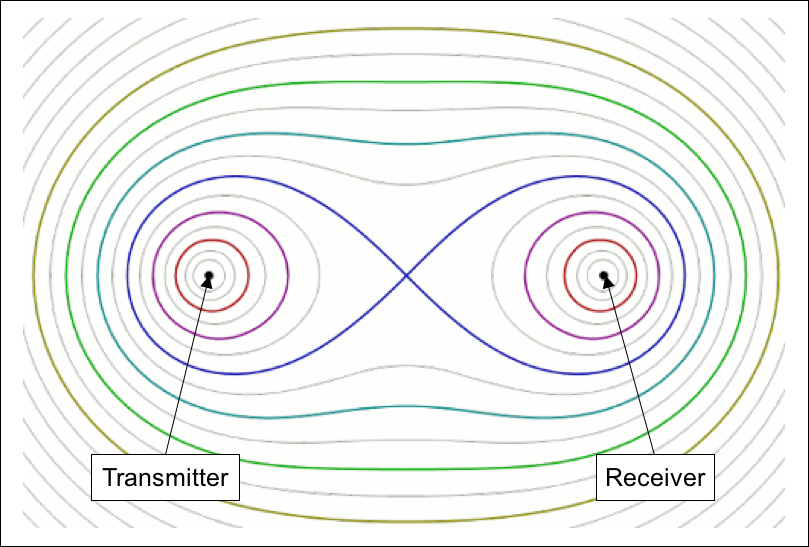
\includegraphics[width=4in]{../media/multistatic/ovals_of_cassini.png}
  \end{center}
  \renewcommand{\baselinestretch}{1} \small\normalsize
  \begin{quote}
    \caption[Ovals of Cassini]{Ovals of Cassini\label{intro_fig:3}}
  \end{quote}
\end{figure}
\renewcommand{\baselinestretch}{2} \small\normalsize
\section{Beam Width}
The beam width of an antenna is defined as the angle between the half power points in the antenna pattern.

\subsection{One Way}
The one way antenna beam width, $\theta$, is simply the beam width of the forward propagating beam.

\subsection{Two Way}
The two way antenna beam width, $\theta_2$, is the beam width of the beam propagating in both directions. For the monostatic case, we can compute this as the one way beam width of the square of the antenna pattern. In most cases, $\theta_2 \approx \frac{1}{\sqrt{2}}\theta$.

\section{Detection}
The detection process can be cast as a hypothesis test where the two mutually exclusive hypotheses are that the target is either present or not present \cite{richards_radar}. There are three probabilities that need to be considered. First, the probability of detection, $P_d$, is the probability that a target is both detected and present. Second, the probability of false alarm, $P_{fa}$ is the probability that a target is detected but not actually present. Finally, the probability of miss, $P_m$ is the probability that a target is present but not detected. In most cases, a missed detection is worse than a false alarm.

\subsection{Threshold Testing}
The detection processes is generally a threshold test applied to the output of a matched filter generated for optimal detection with the threshold, $\hat{T}$ tuned to achieve a specified $P_{fa}$. The received signal consists of thermal noise, potential target returns, and potential interference signals such as clutter or jamming.

Expressions for $P_d$ are complicated but well studied for the cases of standard Gaussian noise and fluctuating targets following Swerling models. In general, $P_d$ is dependent on SNR, so processing is typically geared towards maximizing the SNR. As a general rule of thumb, an SNR of $13$ dB provides a $P_d$ of $\approx 0.94$ and a $P_{fa}$ of $\approx 10^{-6}$.

\subsection{Processing Gains}
To improve the overall SNR and increase the $P_d$, we can take advantage of processing gains by applying the detection strategy to groups of pulses. This is known as pulse integration and we can apply it coherently or noncoherently and can also look at M out of N strategies (binary integration).

\subsubsection{Coherent and Noncoherent Integration}
For coherent integration, we operate in the complex domain and add the magnitude and phase of each pulse. The number of pulses, $N$, that are combined is defined as the Coherent Processing Interval (CPI) and the overall processing gain goes as $N^2$.

For noncoherent integration, we only sum the magnitudes of each pulse. We now refer to th e number of pulses combined, $N$, as the Noncoherent Processing Interval (NPI) and the overall processing gain goes as $N$. When using noncoherent integration, sometimes the NPI is still referred to as the CPI.

Coherently integration $2$ pulses provides a $6$ dB processing gain while noncoherently integrating $2$ pulses only provides a $3$ dB processing gain.

\subsubsection{Binary Integration}